\section{Kết quả huấn luyện mô hình CNN}

\subsection{Kết quả kiểm định chéo 5 phần}

\begin{table}[H]
\centering
\caption{Kết quả kiểm định chéo 5 phần (5-Fold Cross Validation)}
\label{tab:cv_results}
\begin{tabular}{|c|c|c|}
\hline
\textbf{Fold} & \textbf{Accuracy} & \textbf{F1-Score} \\
\hline
Fold 1 & 98.34\% & 98.34\% \\
\hline
Fold 2 & 98.57\% & 98.57\% \\
\hline
Fold 3 & 98.10\% & 98.10\% \\
\hline
Fold 4 & 97.86\% & 97.86\% \\
\hline
Fold 5 & 97.86\% & 97.86\% \\
\hline
\textbf{Mean ± Std} & \textbf{98.15\% ± 0.28\%} & \textbf{98.15\% ± 0.28\%} \\
\hline
\end{tabular}
\end{table}

\textbf{Phân tích kết quả kiểm định chéo:}

Kết quả Cross Validation cho thấy sự ổn định của mô hình: độ lệch chuẩn của Accuracy chỉ khoảng 0.28\%, Accuracy từng fold đều vượt ngưỡng 97.8\%, và điều này cho thấy không có dấu hiệu Overfitting nghiêm trọng, tức Accuracy trên tập validation phản ánh tốt khả năng tổng quát hóa của mô hình.

\begin{figure}[H]
    \centering
    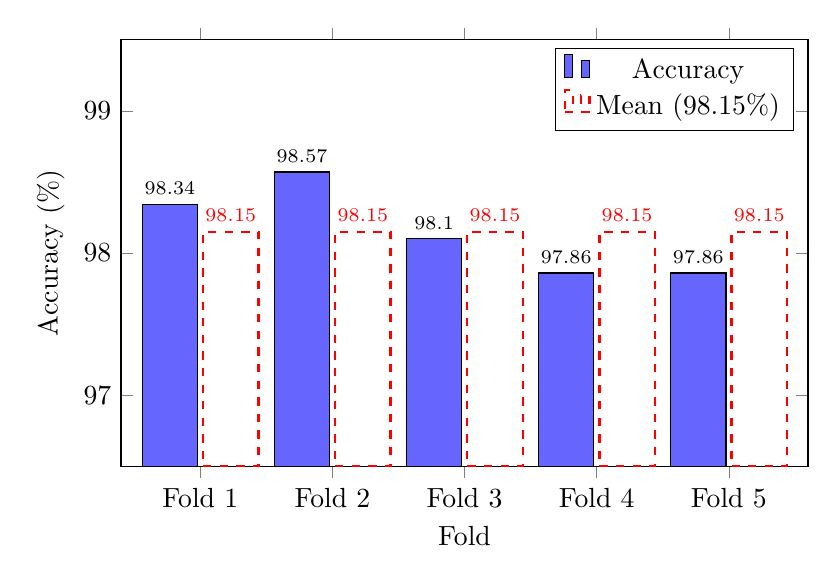
\begin{tikzpicture}
        \begin{axis}[
            ybar,
            width=0.85\textwidth,
            height=7cm,
            ylabel={Accuracy (\%)},
            xlabel={Fold},
            symbolic x coords={Fold 1, Fold 2, Fold 3, Fold 4, Fold 5},
            xtick=data,
            ymin=96.5,
            ymax=99.5,
            bar width=20pt,
            nodes near coords,
            nodes near coords align={vertical},
            every node near coord/.append style={font=\scriptsize},
            enlarge x limits=0.15,
        ]
        \addplot[fill=blue!60] coordinates {
            (Fold 1, 98.34)
            (Fold 2, 98.57)
            (Fold 3, 98.10)
            (Fold 4, 97.86)
            (Fold 5, 97.86)
        };
        % Đường trung bình
        \addplot[red, thick, dashed, domain=0:5] coordinates {
            (Fold 1, 98.15) (Fold 2, 98.15) (Fold 3, 98.15) (Fold 4, 98.15) (Fold 5, 98.15)
        };
        \legend{Accuracy, Mean (98.15\%)}
        \end{axis}
    \end{tikzpicture}
    \caption{So sánh Accuracy giữa các fold trong Cross Validation}
    \label{fig:cv_comparison}
\end{figure}

\subsection{Kết quả trên tập kiểm tra}

\begin{table}[H]
\centering
\caption{Các chỉ số đánh giá trên tập kiểm tra (526 mảnh)}
\label{tab:test_metrics}
\begin{tabular}{|l|c|c|}
\hline
\textbf{Metric} & \textbf{Value} & \textbf{Percent} \\
\hline
\textbf{Accuracy} & 0.9886 & \textbf{98.86\%} \\
\hline
Precision (macro avg) & 0.9886 & 98.86\% \\
\hline
Recall (macro avg) & 0.9886 & 98.86\% \\
\hline
F1-Score (macro avg) & 0.9886 & 98.86\% \\
\hline
ROC-AUC (macro avg) & 0.9998 & 99.98\% \\
\hline
\end{tabular}
\end{table}

\textbf{Ma trận nhầm lẫn trên tập kiểm tra:}

\begin{figure}[H]
    \centering
    \begin{tikzpicture}
        % Định nghĩa màu sắc Blues colormap (từ nhạt đến đậm)
        \definecolor{blue0}{RGB}{247,251,255}
        \definecolor{blue1}{RGB}{222,235,247}
        \definecolor{blue2}{RGB}{198,219,239}
        \definecolor{blue3}{RGB}{158,202,225}
        \definecolor{blue4}{RGB}{107,174,214}
        \definecolor{blue5}{RGB}{66,146,198}
        \definecolor{blue6}{RGB}{33,113,181}
        \definecolor{blue7}{RGB}{8,81,156}
        \definecolor{blue8}{RGB}{8,48,107}

        % Kích thước ô
        \def\cellsize{1.8}

        % Vẽ các ô với màu Blues gradient
        % Hàng 0 (Rừng ổn định): 129, 2, 0, 0
        \fill[blue8] (0*\cellsize, 3*\cellsize) rectangle (1*\cellsize, 4*\cellsize);
        \fill[blue1] (1*\cellsize, 3*\cellsize) rectangle (2*\cellsize, 4*\cellsize);
        \fill[blue0] (2*\cellsize, 3*\cellsize) rectangle (3*\cellsize, 4*\cellsize);
        \fill[blue0] (3*\cellsize, 3*\cellsize) rectangle (4*\cellsize, 4*\cellsize);

        % Hàng 1 (Mất rừng): 4, 126, 0, 0
        \fill[blue1] (0*\cellsize, 2*\cellsize) rectangle (1*\cellsize, 3*\cellsize);
        \fill[blue8] (1*\cellsize, 2*\cellsize) rectangle (2*\cellsize, 3*\cellsize);
        \fill[blue0] (2*\cellsize, 2*\cellsize) rectangle (3*\cellsize, 3*\cellsize);
        \fill[blue0] (3*\cellsize, 2*\cellsize) rectangle (4*\cellsize, 3*\cellsize);

        % Hàng 2 (Phi rừng): 0, 0, 133, 0
        \fill[blue0] (0*\cellsize, 1*\cellsize) rectangle (1*\cellsize, 2*\cellsize);
        \fill[blue0] (1*\cellsize, 1*\cellsize) rectangle (2*\cellsize, 2*\cellsize);
        \fill[blue8] (2*\cellsize, 1*\cellsize) rectangle (3*\cellsize, 2*\cellsize);
        \fill[blue0] (3*\cellsize, 1*\cellsize) rectangle (4*\cellsize, 2*\cellsize);

        % Hàng 3 (Phục hồi rừng): 0, 0, 0, 132
        \fill[blue0] (0*\cellsize, 0*\cellsize) rectangle (1*\cellsize, 1*\cellsize);
        \fill[blue0] (1*\cellsize, 0*\cellsize) rectangle (2*\cellsize, 1*\cellsize);
        \fill[blue0] (2*\cellsize, 0*\cellsize) rectangle (3*\cellsize, 1*\cellsize);
        \fill[blue8] (3*\cellsize, 0*\cellsize) rectangle (4*\cellsize, 1*\cellsize);

        % Vẽ đường viền cho các ô
        \draw[white, line width=1pt] (0,0) grid[step=\cellsize] (4*\cellsize, 4*\cellsize);

        % Thêm số liệu vào các ô
        \node[font=\normalsize\bfseries, text=white] at (0.5*\cellsize, 3.5*\cellsize) {129};
        \node[font=\normalsize, text=black] at (1.5*\cellsize, 3.5*\cellsize) {2};
        \node[font=\normalsize, text=black] at (2.5*\cellsize, 3.5*\cellsize) {0};
        \node[font=\normalsize, text=black] at (3.5*\cellsize, 3.5*\cellsize) {0};

        \node[font=\normalsize, text=black] at (0.5*\cellsize, 2.5*\cellsize) {4};
        \node[font=\normalsize\bfseries, text=white] at (1.5*\cellsize, 2.5*\cellsize) {126};
        \node[font=\normalsize, text=black] at (2.5*\cellsize, 2.5*\cellsize) {0};
        \node[font=\normalsize, text=black] at (3.5*\cellsize, 2.5*\cellsize) {0};

        \node[font=\normalsize, text=black] at (0.5*\cellsize, 1.5*\cellsize) {0};
        \node[font=\normalsize, text=black] at (1.5*\cellsize, 1.5*\cellsize) {0};
        \node[font=\normalsize\bfseries, text=white] at (2.5*\cellsize, 1.5*\cellsize) {133};
        \node[font=\normalsize, text=black] at (3.5*\cellsize, 1.5*\cellsize) {0};

        \node[font=\normalsize, text=black] at (0.5*\cellsize, 0.5*\cellsize) {0};
        \node[font=\normalsize, text=black] at (1.5*\cellsize, 0.5*\cellsize) {0};
        \node[font=\normalsize, text=black] at (2.5*\cellsize, 0.5*\cellsize) {0};
        \node[font=\normalsize\bfseries, text=white] at (3.5*\cellsize, 0.5*\cellsize) {132};

        % Nhãn cột (Dự đoán) - xoay nghiêng
        \node[font=\scriptsize, rotate=45, anchor=east] at (0.5*\cellsize, -0.2*\cellsize) {Rừng ổn định};
        \node[font=\scriptsize, rotate=45, anchor=east] at (1.5*\cellsize, -0.2*\cellsize) {Mất rừng};
        \node[font=\scriptsize, rotate=45, anchor=east] at (2.5*\cellsize, -0.2*\cellsize) {Phi rừng};
        \node[font=\scriptsize, rotate=45, anchor=east] at (3.5*\cellsize, -0.2*\cellsize) {Phục hồi rừng};
        \node[font=\small\bfseries] at (2*\cellsize, -1.1*\cellsize) {Dự đoán};

        % Nhãn hàng (Thực tế)
        \node[font=\scriptsize, anchor=east] at (-0.1*\cellsize, 3.5*\cellsize) {Rừng ổn định};
        \node[font=\scriptsize, anchor=east] at (-0.1*\cellsize, 2.5*\cellsize) {Mất rừng};
        \node[font=\scriptsize, anchor=east] at (-0.1*\cellsize, 1.5*\cellsize) {Phi rừng};
        \node[font=\scriptsize, anchor=east] at (-0.1*\cellsize, 0.5*\cellsize) {Phục hồi rừng};
        \node[font=\small\bfseries, rotate=90] at (-1.5*\cellsize, 2*\cellsize) {Thực tế};

        % Thanh màu (color bar) - Blues gradient (9 segments, mỗi segment = 4/9 cellsize)
        \pgfmathsetmacro{\segheight}{4/9}
        \foreach \i/\col in {0/blue0, 1/blue1, 2/blue2, 3/blue3, 4/blue4, 5/blue5, 6/blue6, 7/blue7, 8/blue8} {
            \fill[\col] (5*\cellsize, \i*\segheight*\cellsize) rectangle (5.4*\cellsize, \i*\segheight*\cellsize+\segheight*\cellsize);
        }
        \draw[black, thin] (5*\cellsize, 0) rectangle (5.4*\cellsize, 4*\cellsize);
        \node[font=\tiny, anchor=west] at (5.5*\cellsize, 0) {0};
        \node[font=\tiny, anchor=west] at (5.5*\cellsize, 1*\cellsize) {40};
        \node[font=\tiny, anchor=west] at (5.5*\cellsize, 2*\cellsize) {80};
        \node[font=\tiny, anchor=west] at (5.5*\cellsize, 3*\cellsize) {120};
    \end{tikzpicture}
    \caption{Confusion Matrix dạng heatmap trên tập kiểm tra (n=526, Accuracy: 98.86\%)}
    \label{fig:confusion_heatmap}
\end{figure}

\textbf{Phân tích chi tiết từng lớp trên tập kiểm tra:}

\begin{table}[H]
\centering
\caption{Phân tích chi tiết từng lớp}
\label{tab:class_analysis}
\begin{tabular}{|l|c|c|c|c|c|}
\hline
\textbf{Lớp} & \textbf{Precision} & \textbf{Recall} & \textbf{F1-Score} & \textbf{Samples} & \textbf{Errors} \\
\hline
0 - Rừng ổn định & 96.99\% & 98.47\% & 97.73\% & 131 & 4 FP, 2 FN \\
\hline
1 - Mất rừng & 98.44\% & 96.92\% & 97.67\% & 130 & 2 FP, 4 FN \\
\hline
2 - Phi rừng & 100.00\% & 100.00\% & 100.00\% & 133 & 0 \\
\hline
3 - Phục hồi rừng & 100.00\% & 100.00\% & 100.00\% & 132 & 0 \\
\hline
\end{tabular}
\end{table}

\textit{Ghi chú: FP = False Positive (dương tính giả), FN = False Negative (âm tính giả)}

\textbf{Phân tích lỗi phân loại:}

Tổng cộng chỉ có 6/526 mẫu bị phân loại sai, tương đương tỷ lệ lỗi 1.14\%. Trong đó, hai mẫu thuộc Lớp 0 (Rừng ổn định) bị nhầm thành Lớp 1 (Mất rừng) và bốn mẫu thuộc Lớp 1 (Mất rừng) bị nhầm thành Lớp 0 (Rừng ổn định). Đánh giá chi tiết cho thấy Lớp 2 (Phi rừng) và Lớp 3 (Phục hồi rừng) được phân loại hoàn hảo với Accuracy 100\%.

\textbf{Phân tích nguyên nhân nhầm lẫn giữa Rừng ổn định và Mất rừng:}

Việc nhầm lẫn chỉ xảy ra giữa hai lớp Rừng ổn định (Lớp 0) và Mất rừng (Lớp 1) có thể được giải thích bởi các yếu tố sau:

\begin{itemize}
    \item \textbf{Sự tương đồng về đặc trưng quang phổ:} Cả hai lớp đều có sự hiện diện của rừng ở ít nhất một thời điểm. Các khu vực rừng bị suy thoái nhẹ có thể có phổ phản xạ đặc trưng tương tự với rừng ổn định, đặc biệt khi mức độ mất rừng không rõ ràng.

    \item \textbf{Hiệu ứng biên:} Tại ranh giới giữa vùng rừng và vùng mất rừng, các điểm ảnh có thể chứa cả hai loại lớp phủ (điểm ảnh hỗn hợp), dẫn đến vector đặc trưng không điển hình cho một lớp cụ thể.

    \item \textbf{Biến động theo mùa:} Một số khu vực rừng ngập mặn có thể có biến động theo mùa về mật độ tán lá, tạo ra sự thay đổi NDVI tương tự như mất rừng nhưng thực tế là biến động tự nhiên.

    \item \textbf{Độ phân giải thời gian:} Với chỉ hai thời điểm quan sát, một số biến động ngắn hạn hoặc phục hồi nhanh có thể không được ghi nhận chính xác.
\end{itemize}

Tuy nhiên, với tỷ lệ nhầm lẫn rất thấp (chỉ 6/526 mẫu, ~1.14\%), mô hình vẫn đạt hiệu quả cao trong việc phân biệt các lớp biến động rừng.

\subsection{Đường cong ROC}

\begin{table}[H]
\centering
\caption{Điểm ROC-AUC cho từng lớp trên tập kiểm tra}
\label{tab:roc_auc}
\begin{tabular}{|l|c|}
\hline
\textbf{Lớp} & \textbf{ROC-AUC} \\
\hline
0 - Rừng ổn định & 0.9998 \\
\hline
1 - Mất rừng & 0.9997 \\
\hline
2 - Phi rừng & 1.0000 \\
\hline
3 - Phục hồi rừng & 1.0000 \\
\hline
\textbf{Trung bình macro} & \textbf{0.9998} \\
\hline
\end{tabular}
\end{table}

\begin{figure}[H]
    \centering
    \begin{tikzpicture}
        \begin{axis}[
            width=0.75\textwidth,
            height=8cm,
            xlabel={False Positive Rate (FPR)},
            ylabel={True Positive Rate (TPR)},
            xmin=0, xmax=1,
            ymin=0, ymax=1,
            legend pos=south east,
            legend style={font=\small},
            grid=major,
            grid style={dashed, gray!30},
        ]
        % Đường chéo (phân loại ngẫu nhiên)
        \addplot[gray, dashed, thick] coordinates {(0,0) (1,1)};

        % Đường cong ROC cho 4 lớp (mô phỏng dựa trên AUC cao)
        % Lớp 0 - Rừng ổn định (AUC = 0,9998)
        \addplot[green!60!black, thick] coordinates {
            (0,0) (0,0.95) (0.001,0.98) (0.002,0.99) (0.01,0.995) (0.05,0.998) (1,1)
        };
        % Lớp 1 - Mất rừng (AUC = 0,9997)
        \addplot[red!70, thick] coordinates {
            (0,0) (0,0.94) (0.001,0.97) (0.003,0.99) (0.01,0.994) (0.05,0.997) (1,1)
        };
        % Lớp 2 - Phi rừng (AUC = 1,0000)
        \addplot[blue!60, thick] coordinates {
            (0,0) (0,1) (1,1)
        };
        % Lớp 3 - Phục hồi rừng (AUC = 1,0000)
        \addplot[orange!80, thick] coordinates {
            (0,0) (0,1) (1,1)
        };

        \legend{Ngẫu nhiên, Rừng ổn định, Mất rừng, Phi rừng, Phục hồi rừng}
        \end{axis}
    \end{tikzpicture}
    \caption{Đường cong ROC cho các lớp phân loại}
    \label{fig:roc_curves}
\end{figure}